% arara: pdflatex: {synctex: yes}
% arara: makeindex: { style: SpecificImpulseEff }
% arara: biber
% arara: pdflatex: {synctex: yes}
% arara: pdflatex: {synctex: yes}
% arara: clean: {files: [SpecificImpulseEff.aux, SpecificImpulseEff.idx, SpecificImpulseEff.ilg, SpecificImpulseEff.ind, SpecificImpulseEff.log, SpecificImpulseEff.bbl, SpecificImpulseEff.bcf, SpecificImpulseEff.ist, SpecificImpulseEff.blg, SpecificImpulseEff.run.xml]}
%
\documentclass[]{memoir} %twocolumn
\usepackage[utf8]{inputenc}
\usepackage[english]{babel}
\usepackage[T1]{fontenc}
% Nicer default font (+ math font) than Computer Modern for most use cases
\usepackage{mathpazo}
\usepackage[labelfont=bf]{caption}
\usepackage{xcolor} % Allow colors to be defined
\usepackage{enumerate} % Needed for markdown enumerations to work
\usepackage[]{geometry} % Used to adjust the document margins
\usepackage{amsmath} % Equations
\usepackage{amssymb} % Equations
\usepackage{booktabs}  
\usepackage{longtable}
\usepackage{wrapfig}
\usepackage{dblfloatfix}
\usepackage{tikz} 
\usepackage{pgf}
\usepackage{float}
\usepackage[pdftex,colorlinks]{hyperref}
\usepackage[noabbrev, capitalize]{cleveref}
\usepackage[shortlabels]{enumitem}

\providecommand{\tightlist}{%
  \setlength{\itemsep}{0pt}\setlength{\parskip}{0pt}
}

\renewcommand*\familydefault{\sfdefault}

\chapterstyle{demo2}
\setlrmarginsandblock{0.75in}{0.75in}{*}
\setulmarginsandblock{1in}{*}{1}
\checkandfixthelayout 

\usepackage{graphicx}
\graphicspath{{./imgs/}}

\title{AA103 Final Project}
\author{Jonny Dyer}
 
\begin{document}

\chapter*{AA103 Final Project}

\section{Project Description}
For our final project, you will be designing, building and launching a water rocket!

Water rockets are generally made from 2 liter soda bottles filled partially with water and
pressurized with air.  The water is exhausted through a nozzle creating thrust and
launching the bottle into the sky.  There is a vibrant group of garage builders on
the internet and some hava achieved amazing performance,
\href{http://www.wra2.org/WRA2_Standings.php}{flying rockets to over 2000
feet in altitude}! (albeit not with soda bottles...)  

\begin{figure}[H]
    \centering
    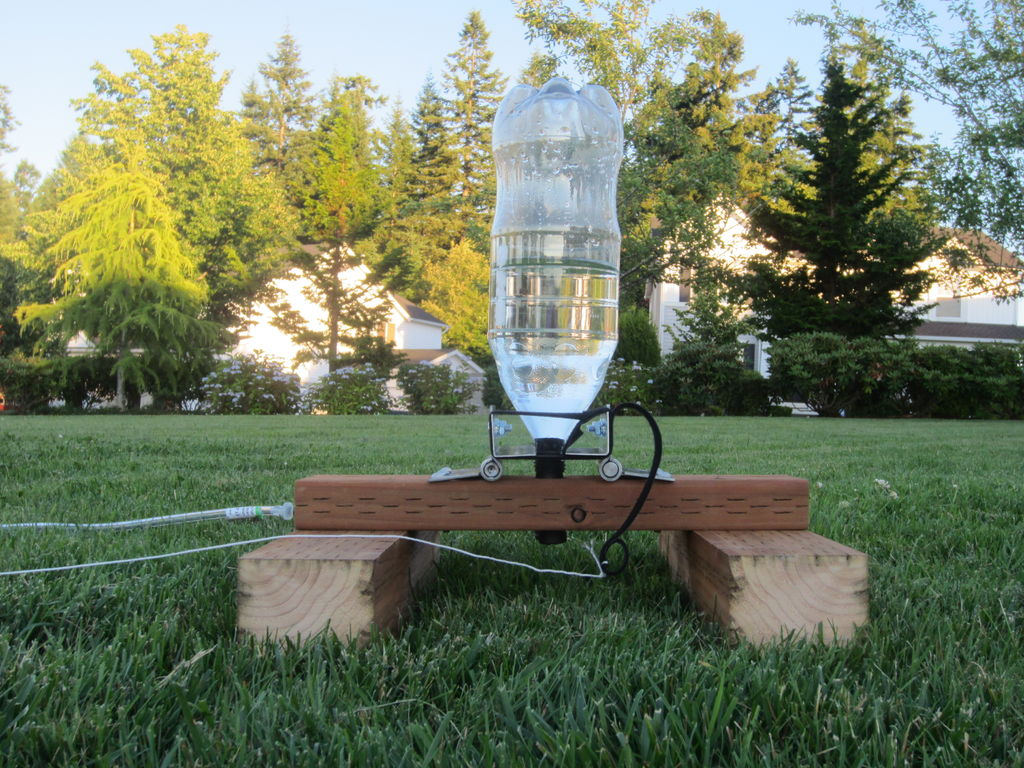
\includegraphics[width=0.95\columnwidth]{water_rocket}
\end{figure}

While without smoke and fire, water rockets are a lot of fun.  

This project is broken into two parts:

\begin{enumerate}
    \item Pre-work problem set covering the analysis and design of the rocket
    \item The rocket build and altitude contest
\end{enumerate}

\subsection{Rules and Constraints}

Since we will be holding a contest, there are some rules and constraints that must be followed:

\begin{itemize}
    \item Everyone must use a standard 2 liter soda bottle.  The beverage choice is up to you...
    \item All rockets will be pressurized to 7 bar (1 bar is $1\times10^5$ Pa)
    \item All rockets will carry a 10 g altimeter payload on top
    \item All rockets must use the provided bottle cap / nozzle.  However, the nozzle internal
        hole may be modified by the teams
\end{itemize}

\section{Pre-work - Analysis and Design}

\subsection{Problem 1 - $\Delta V$ analysis}
Firs we will ask you to compute the $\Delta V$ your rocket is capable of delivering.  A water 
rocket is referred to as a "blow-down" system as there is no external reservoir of propellant
maintaining constant pressure in the rocket.  So the pressure inside will decay as water is
expelled. 

In general terms, a gas expansion process can be represented as

\begin{equation}
    pV^n = \text{const}
\end{equation}

\begin{enumerate}[a)]
    \item What is $n$ for the three following processes?

    \begin{enumerate}
        \item An Isobaric (constant pressure) process
        \item An Isothermal (constant temperature) process
        \item An Isentropic (constant entropy) process
    \end{enumerate}

    \item Given that a water rocket expels the water in a very short period of time (a second or two) and
            that the gas must perform work on the water in this expulsion, which type of process above do you
            think most accurately models the expansion process of the gas?

    \item Given an initial internal pressure, $p_0 = 7$ bar, an ambient atmospheric pressure, $p_a = 1$ bar,
        and the density of water $rho_w = 1000 kg/m^3$ what is the initial water exit velocity?

    \item If the expulsion process were isobaric, derive the rocket $\Delta V$ as a function of \emph{water
        fill fraction}, $\alpha = \frac{V_w}{V_t}$ where $V_w$ is the volume of the bottle initially filled
        with water and $V_t$ is the total volume of the bottle.  You may assume the mass of your bottle is
        50g plus 15g for the altimeter payload.

    \item Since the explusion process is not really isobaric, we would like to derive the $\Delta V$ for
        the isothermal and isentropic cases as well. Unfortunately, there is not a closed form solution
        for this so we will need to compute a differential equation for velocity increment and then 
        integrate numerically.  The jupyter notebook linked gives the background necessary to do this integration.

    \item Given the results from this analysis, how would you pick the fill fraction $\alpha$?  How different
        is your answer for the isothermal and isentropic cases?
\end{enumerate}

\subsection{Problem 2 - Ballistic simulation and optimization}

In the previous problem we looked at $\Delta V$ potential of your rocket.  This is interesting and 
informative but it neglects to consider two unfortunate facts:

\begin{enumerate}
    \item Your rocket must fight gravity
    \item Your rocket will be slowed by aerodynamic drag
\end{enumerate}

In this problem you will develop a very simple numerical simulation of the rocket's flight trajectory
and use this to interogate its performance sensitivity to some design parameters.

\bibliographystyle{unsrt}
\bibliography{refs}

\end{document}
